\documentclass[10pt,reqno]{beamer}
\usepackage[utf8]{inputenc}
\usepackage[LGR,T1]{fontenc}
\usetheme{Dresden}
\usecolortheme{beaver}
\usepackage{amsmath}
\usepackage{amsthm}
\usepackage{amsfonts}
\usepackage{graphicx}
\usepackage{animate}
\usepackage[absolute,overlay]{textpos}
\usepackage{calc}
\usepackage{xcolor}
\usepackage{tcolorbox}
\usepackage[style=authoryear, natbib=true, autocite=superscript]{biblatex}
\usepackage{appendixnumberbeamer}
\bibliography{../references/synch_master}
\newcommand{\D}[2]{\frac{\mathrm{d} #1}{\mathrm{d} #2}}
\newcommand{\e}{\mathrm{e}}
\newcommand{\I}{\mathrm{i}}
\renewcommand{\mod}[1]{\left|#1\right|}
\newcommand{\textgreek}[1]{\begingroup\fontencoding{LGR}\selectfont#1\endgroup}
\newcommand{\DD}[2]{\frac{\mathrm{d}^2 #1}{\mathrm{d} #2^2}}
\newcommand{\bigO}[1]{\text{O}\left(#1\right)}
\renewcommand{\P}[2]{\frac{\partial #1}{\partial #2}}
\renewcommand{\Re}{\operatorname{Re}}
\renewcommand{\Im}{\operatorname{Im}}
\newcommand{\EX}{\mathbb{E}}
\newcommand{\df}[1]{\mspace{2mu}  \mathrm{d}#1}
\newcommand{\reals}{\mathbb{R}}
\newcommand{\complex}{\mathbb{C}}
\newcommand{\conj}[1]{\overline{#1}}
\definecolor{lred}{rgb}{1,0.8,0.8}
\newcommand{\highlight}[1]{\colorbox{lred}{$\displaystyle #1$}}
\newcommand{\iip}[2]{\langle #1,#2\rangle}
\newcommand{\ip}[2]{\left\langle #1,#2\right\rangle}

\graphicspath{{../images/synch/}{../images/logos/}}
\newcommand{\github}{\url{https://github.com/peter-cudmore/seminars/}}
\setbeamercolor{blockcl}{fg=black,bg=lred}
\textblockorigin{\paperwidth}{9.5mm}

\def\overlay1 {\begin{textblock}{5}[1,0](0,-0.25)\[F(r)=[f(1+\I\Omega)]^{-1}\]\end{textblock}}
%
%\DeclareCiteCommand{\cite}
%{\usebibmacro{prenote}}%
%{%  
%	\ifciteseen{}{%
%		\usebibmacro{citeindex}%
%		\let\thefootnote\relax%
%		\footnotetext{%
%			\scriptsize
%			\mkbibbrackets{\usebibmacro{cite}}%
%			\setunit{\addnbspace}
%			\printnames{labelname}%
%			\setunit{\labelnamepunct}
%			\printfield[citetitle]{title}%
%			\newunit%
%			\printfield[]{year}%
%		}%
%		\let\thefootnote\svthefootnote%
%	}%
%	\autocite{\thefield{entrykey}}%
%}
%{\addsemicolon\space}
%{\usebibmacro{postnote}}
\renewbibmacro*{cite}{%
	\iffieldundef{shorthand}
	{\ifthenelse{\ifnameundef{labelname}\OR\iffieldundef{labelyear}}
		{\usebibmacro{cite:label}%
			\setunit{\addspace}}
		{\printnames{labelname}%
			\setunit{\nameyeardelim}}%
		\usebibmacro{cite:labelyear+extrayear}%
		\setunit{\addcomma\space}%
		\usebibmacro{journal}}
	{\usebibmacro{cite:shorthand}}}

\makeatletter
\setbeamertemplate{footline}
{%
	\begin{beamercolorbox}[colsep=1.5pt]{upper separation line foot}
	\end{beamercolorbox}
	\begin{beamercolorbox}[ht=2.5ex,dp=1.125ex,%
		leftskip=.3cm,rightskip=.3cm plus1fil]{author in head/foot}%
		\leavevmode{\usebeamerfont{author in head/foot}\insertshortauthor}%
		\hfill%
		{\usebeamerfont{institute in head/foot}\usebeamercolor[fg]{institute in head/foot}\insertshortinstitute}%
	\end{beamercolorbox}%
	\begin{beamercolorbox}[ht=2.5ex,dp=1.125ex,%
		leftskip=.3cm,rightskip=.3cm plus1fil]{title in head/foot}%
		{\usebeamerfont{title in head/foot}\insertshorttitle}%
		\hfill%
		{\usebeamerfont{title in head/foot}\github}
	\end{beamercolorbox}%
	\begin{beamercolorbox}[colsep=1.5pt]{lower separation line foot}
	\end{beamercolorbox}
}
\makeatother


\setbeamertemplate{navigation symbols}{} 
\title{Synchronisation of Nonlinearly Coupled Oscillators}

\author{Peter Cudmore}
\titlegraphic{
\includegraphics[scale=0.5]{PRIMARY_A_Vertical_Housed_RGB.png}}
\institute{University of Melbourne}
\date{\today}

%\AtBeginSection[] { 
%\begin{frame}
%\tableofcontents[currentsection,hideallsubsections] 
%\addtocounter{framenumber}{-1} 
%\end{frame}
%}

\begin{document}

\begin{frame}
\titlepage
\addtocounter{framenumber}{-1} 

\end{frame}
%\section{Nonlinearly Coupled Oscillators.}

\begin{frame}
\frametitle{Acknowledgements}
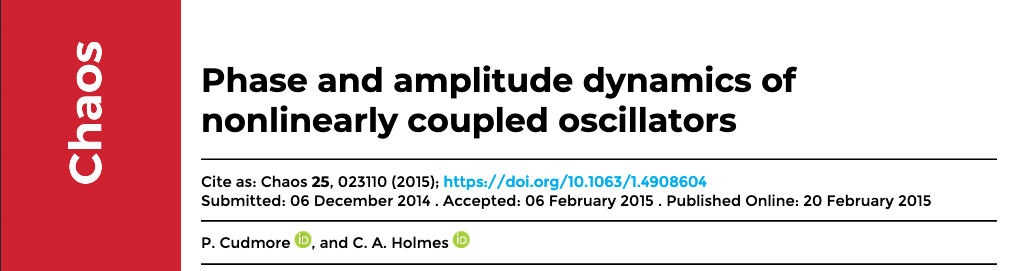
\includegraphics[width=0.8\linewidth]{chaosss}
\vfill
{\scriptsize The research presented was performed under the supervision of Dr. Catherine A. Holmes, Prof. Joseph Grotowski and Dr. Cecilia Gonz\`ales Tokman at the University of Queensland (UQ) as part the doctoral program funded under the Australian Postgraduate Award and Discovery Early Career Researcher Award: DE160100147.}\\
\vfill

\includegraphics[width=\linewidth]{uqarc}	
\end{frame}
\begin{frame}
\frametitle{Coupled Oscillators in Nature}
Oscillatory systems are common in nature and the physical sciences. For example:
\begin{itemize}
	\item Fireflies in South East Asia,
	\item Circadian Rhythms,
	\item Neural Oscillations,
	\item Semiconductor Physics (Josephson Junctions), 
	\item {\em Quantum Nanotechnology}.
\end{itemize}
When many individual oscillators are coupled, allowing each oscillator to influence some (or all) others, surprising emergent phenomenon can occur.

In particular such systems can exhibit {\em synchronisation}!
\end{frame}
\begin{frame}
\frametitle{Synchronisation: a universal phenomenon.}
\begin{center}
{\em Synchronisation} occurs when mutual interactions cause a portion of the individual oscillators to move in unison.
\end{center}
\begin{columns}
\begin{column}{0.49\textwidth}
	\begin{figure}
		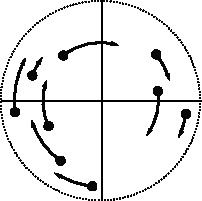
\includegraphics[scale=0.80]{synch1.pdf}
		\caption{Unsynchronised motion: oscillators rotate at different angular velocities.}
	\end{figure}
\end{column}
\begin{column}{0.49\textwidth}
	\begin{figure}
		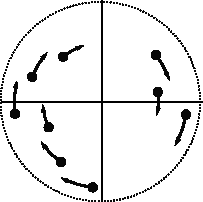
\includegraphics[scale=0.80]{synch2.pdf}
		\caption{Synchronised motion: all oscillators rotate at the same angular velocity.}
	\end{figure}
\end{column}
\end{columns}
\end{frame}
\begin{frame}
\frametitle{Nano-electromechanics: A future technology.}
Nano-electromechanical systems(NEMS) have potential applications in the measurement of weak forces (gravitational waves, single atom charge/spin),
quantum computing (switches, memory) and exploration below the quantum limit.
\begin{figure}
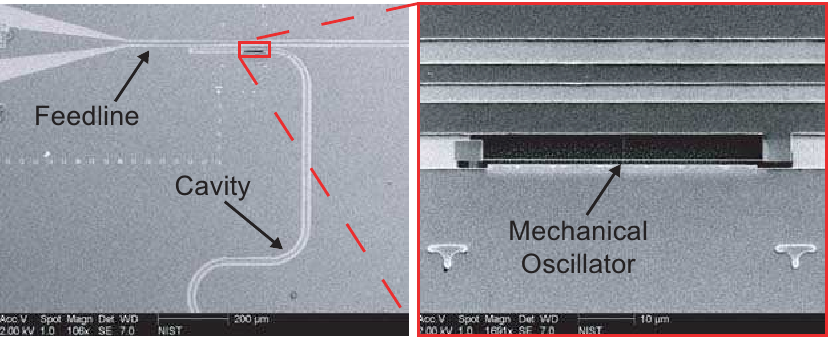
\includegraphics[scale=0.35]{cavity.jpg}
\caption{A Nano-electromechanical system. \footcite{nanoimg}}
\end{figure}
\end{frame}
\begin{frame}
\frametitle{NEMS as a coupled oscillator system.}
\begin{figure}
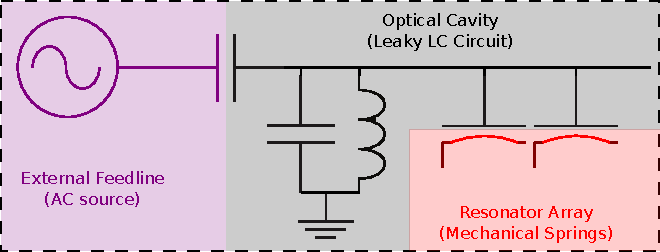
\includegraphics[scale=0.7]{schem2.pdf}
\caption{Semiclassical model of a NEMS.}
\end{figure}
\begin{itemize}
\item Mean spring displacement modulates the circuits resonant frequency.
\item Photon-phonon interaction forces springs.
\item {\em Nonlinear all-to-all coupling between mechanical oscillators}.
\end{itemize}
\end{frame}

\begin{frame}[t]
\frametitle{Oscillators in $\complex$.} 
Consider a set (or population) of $n$ damped harmonic oscillators $\{z_j\}$;
\[
\D{z_j}{t} =(-1+\I\omega_j)z_j. \qquad j=1,\ldots,n
\] 
\begin{minipage}{0.49\textwidth}
Each oscillator $z_j$ has:
\begin{itemize}
\item Phase $\arg{z_j}$,
\item amplitude $\mod{z_j}$ and 
\item natural frequency $\omega_j$.
\end{itemize}
~\\
Each $\omega_j$ is a real valued I.I.D random variable with density $g(\omega)$.
\end{minipage}
\begin{minipage}{0.49\textwidth}
\begin{figure}
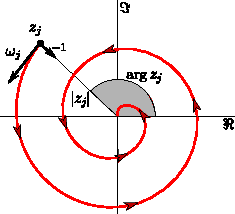
\includegraphics[scale = 0.95]{dosc}
\end{figure}
\centering
$z_j(t) = z_j(0)\exp[(-1+\I\omega_j)t]$
\end{minipage}
\end{frame}
\begin{frame}
\frametitle{Population mean as a measure of coherence.}
We can measure the state of the population by observing the population mean, or {\em order parameter} \footcite{kuramoto75}:
\[
z = \frac{1}{n}\sum_{j=1}^n z_j
\]
\begin{columns}
\begin{column}{0.59\textwidth}
We call:
\begin{itemize}
\item $z$ the {\em mean field}.
\item $r=\mod{z}$ the mean field amplitude.
\item $\Theta = \arg{z}$ the mean phase.
\item $\Omega = \D{\Theta}{t}$ the mean field velocity.
\end{itemize}
\end{column}
\begin{column}{0.39\textwidth}
\begin{figure}
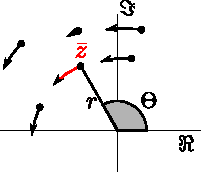
\includegraphics{meanfield.pdf}
\end{figure}
\end{column}
\end{columns}
\end{frame}

\begin{frame}
\frametitle{A more general model: The Hopf Bifurcation}
The normal form of a Hopf Bifurcation at $\alpha = 0$ is given by
\[
\D{z_j}{t}= (\alpha - \beta\mod{z_j}^2)z + \I\omega_j z_j, \qquad \beta >0.
\]
\begin{columns}[t]
\begin{column}{.49\textwidth}
\centering
$\alpha <0$
\begin{figure}
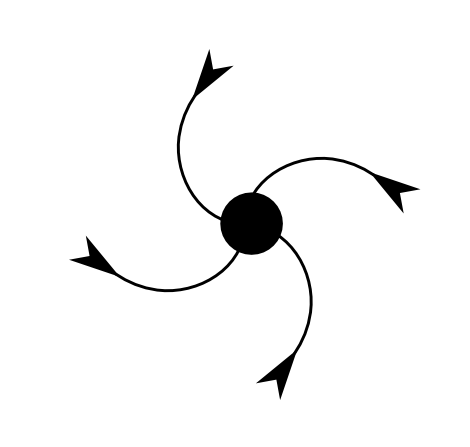
\includegraphics[scale = 0.16]{node.png}
\end{figure}
When $\alpha \le 0$ the fixed point at $z_j =0$ is stable.
\end{column}
\begin{column}{.49\textwidth}
\centering
$\alpha >0$
\begin{figure}
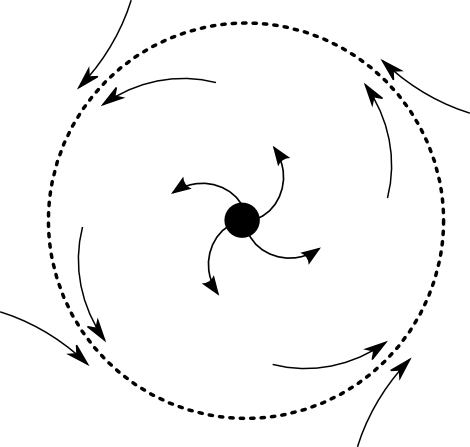
\includegraphics[scale = 0.16]{hopf.png}
\end{figure}
For $\alpha>0$, the $z_j=0$ state is unstable and a stable limit cycle exists with $\mod{z_j} = \sqrt{\alpha/\beta}$				
\end{column}
\end{columns}
\end{frame}
\begin{frame}
\frametitle{Coupled Oscillator Systems on either side of a Hopf}
\begin{columns}[t]
\only<1>{
\begin{column}{.49\textwidth}
\centering
Linear Oscillator Model:
\[
\D{z_j}{t} = (\alpha +\I\omega_j)z_j+\Gamma(z)
\]
$\alpha <0,\ j = 1\dots n$.
\begin{figure}
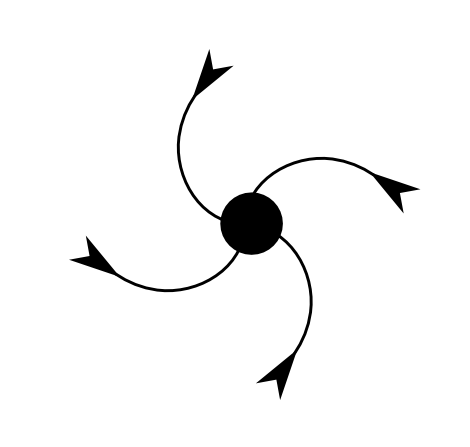
\includegraphics[scale = 0.16]{node.png}
\end{figure}
Decoupled system has a stable node and no stable limit cycles.
\end{column}}
\only<1-2>{
\begin{column}{.49\textwidth}
\centering
Limit Cycle Model:
\[
\D{z_j}{t} = (\alpha - \beta|z_j|^2)z_j + \I\omega_jz_j +\Gamma(z)
\]
$\alpha,\beta>0, j = 1\dots n$
\begin{figure}
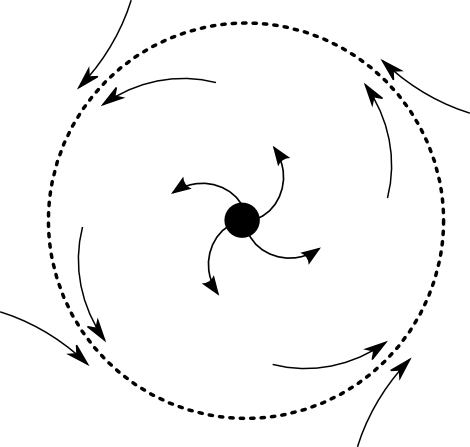
\includegraphics[scale = 0.16]{hopf.png}
\end{figure}
Decoupled system has unstable node and a stable limit cycle.
\end{column}}
\only<2>{
\begin{column}{.49\textwidth}
{\em The Kuramoto Model}.
\[
\D{\theta_j}{t} = \omega_j  + \frac{\gamma}{n}\sum_{k=1}^N\sin(\theta_k - \theta_j) 
\]
\vspace{10pt}\\
Literature includes work by
\begin{itemize}
\item Y. Kuramoto,
\item S. Strogatz \& R. Mirollo,
\item M. Cross,
\item A. Pikovsky \& M. Rosenblum,
\item G. Ermentrout and
\item D. Aronson \& more..
\end{itemize}
\end{column}}
\end{columns}
\end{frame}
\begin{frame}
\frametitle{Synchronisation of Limit Cycle Oscillators}
\begin{center}
A common theme is that synchronisation occurs due to a {\em play-off between frequency spread and coupling strength}.
\end{center}
\begin{figure}
\animategraphics[autoplay,loop,height=5cm]{6}{anims/lcsynch-}{1}{100}
\end{figure}
\end{frame}

\begin{frame}[t]
\frametitle{Linear oscillators with nonlinearly coupling.}
We are concerned with nonlinear all-to-all coupling via the mean field
\[
\D{z_j}{t} = -(1-\I\omega_j)z_j + zF(\mod{z}), \qquad z= \frac{1}{n}\sum_{j=1}^n z_j
\] 
\begin{itemize}
\item $\omega_j$ are I.I.D. with a p.d.f given by $g(\omega)$.
\item Coupling is linear in mean field phase;
\item and nonlinear in mean field amplitude.
\item Nonlinear coupling function $F :C^1 [0,\infty) \rightarrow \complex$. 
\item {\em Nonlinearly coupled oscillators are not well understood.}
\end{itemize}
\end{frame}
\begin{frame}
\frametitle{Identical oscillators follow mean field}
It has been shown\footcite{Cathy2012} that if $\omega_j=\omega$ then 
in the steady state $z_j=z$ and 
\[
\D{z}{t}= -(1-\I\omega)z + zF(\mod{z}).
\] 
\begin{columns}
\begin{column}{0.59\textwidth}
In polar form:
\begin{eqnarray*}
\D{r}{t} &=& -r[1-\Re F(r)],\\
\Omega &=& \omega + \Im F(r).
\end{eqnarray*}
\begin{itemize}
\item $\Omega$ constant implies $\D{r}{t}=0$.
\item Fixed points at $r=0$ \& $\Re F(r)=1$.
\item {\em Phase and amplitude decouple!}
\end{itemize}
\end{column}
\begin{column}{0.39\textwidth}
\begin{figure}
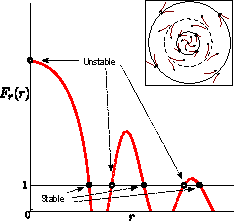
\includegraphics{identical.pdf}
\end{figure}
\end{column}
\end{columns}
\end{frame}
\begin{frame}
\frametitle{Non-identical case: does synchronisation occur?}
Key questions for the non-identical case:
\begin{itemize}
\item Can nonlinear coupling destabilise the origin?
\item Does this system have stable synchronised solutions?
\item Can this system have {\em multiple} stable synchronised states?
\end{itemize}
\vspace{10pt}
The answer: yes!\footcite{pc2015} (but it would take more than ten minutes to explain).
\end{frame}
\begin{frame}[t]
\frametitle{`Shape' of $F$ and $g$ are bifurcations parameters.}
We can, with generality, identify existence, stability and bifurcations of synchronised solutions in the non-identical case.\\~\\
{\em A bifurcation occurs when a small smooth change made to the parameter values (the bifurcation parameters) of a system causes a sudden `qualitative' or topological change in its behaviour.}
\\~\\
Bifurcation parameters for this system:
\begin{itemize}
\item The `shape' of coupling function $F(r)$ (e.g.; coefficients of nonlinearities).  
\item The `shape' of the distribution $g(\omega)$ (e.g.; spread, number of modes).
\end{itemize}
\end{frame}
\begin{frame}
\frametitle{'Unsynchronised' Motion}
\begin{textblock}{1}[1,0](-2.8,2)
\animategraphics[autoplay,loop,height=20mm]{15}{anims/unsynchs-}{1}{100}
\end{textblock}
\begin{figure}
\animategraphics[autoplay,loop,height=0.62\paperheight,width=0.8\paperwidth]{10}{anims/unsynch-}{1}{100}
\end{figure}
\end{frame}
\begin{frame}
\frametitle{Synchronisation}
\begin{textblock}{1}[1,0](-2.8,2)
\animategraphics[autoplay,loop,height=20mm]{15}{anims/synchs-}{1}{100}
\end{textblock}
\begin{figure}
\animategraphics[autoplay,loop,height=0.62\paperheight,width=0.8\paperwidth]{10}{anims/synch-}{1}{100}
\end{figure}
\end{frame}
\begin{frame}
\frametitle{Density on real line to density on a circle}
\begin{textblock}{1}[1,0](-0.8,-0.5)
\animategraphics[autoplay,loop,height=10mm]{15}{anims/lsynch-}{1}{25}
\end{textblock}

\begin{figure}
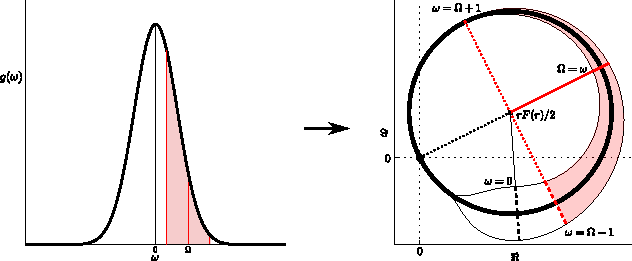
\includegraphics[scale=0.95]{dist}
\caption{In the fixed state, the density $g$ is mapped to a density on the circle represented by the shaded area. 
Oscillators with $\omega \in (\Omega-1, \Omega+1)$ are mapped to the shaded region furthest from the origin.}
\end{figure}
\end{frame}
\begin{frame}
\frametitle{Some different distributions}
\begin{textblock}{1}[1,0](-0.8,-0.5)
\animategraphics[autoplay,loop,height=10mm]{15}{anims/lsynch-}{1}{25}
\end{textblock}

\begin{figure}
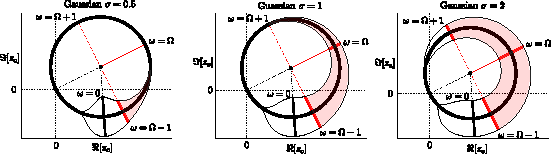
\includegraphics{gaussiancomp}
\end{figure}

\begin{figure}
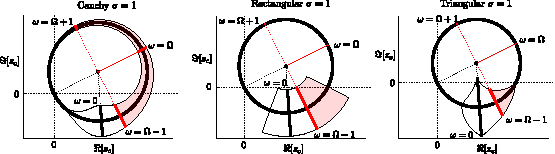
\includegraphics{distcomp}
\end{figure}


\end{frame}
\begin{frame}
\frametitle{Conclusions}
Synchronised states exist systems consisting of linear oscillators with nonlinear coupling.\\
These system are different to much of those in coupled oscillator literature as:
\begin{itemize}
\item The amplitude dynamics are important.
\item The individual oscillators are linear.
\item The coupling is nonlinear. 
\end{itemize}

In particular, synchronise solutions exist on a regular pattern, and this pattern is related to the distribution of oscillator frequencies.
\begin{textblock}{1}[1,0](-0.8,-0.5)
\animategraphics[autoplay,loop,height=10mm]{15}{anims/lsynch-}{1}{25}
\end{textblock}

\end{frame}
\appendix
\begin{frame}[allowframebreaks]
\frametitle{References}
\footnotesize
\printbibliography
\end{frame}

\end{document}
